\paragraph{Sơ đồ tuần tự luồng Kích hoạt xác thực 2 lớp}

Luồng nghiệp vụ này mô tả
chi tiết quá trình người dùng
thiết lập mã xác thực hai lớp (2FA)
sử dụng giao thức TOTP (Time-based One-Time Password)
qua Supabase Auth Service.

\begin{figure}[H]
\centering
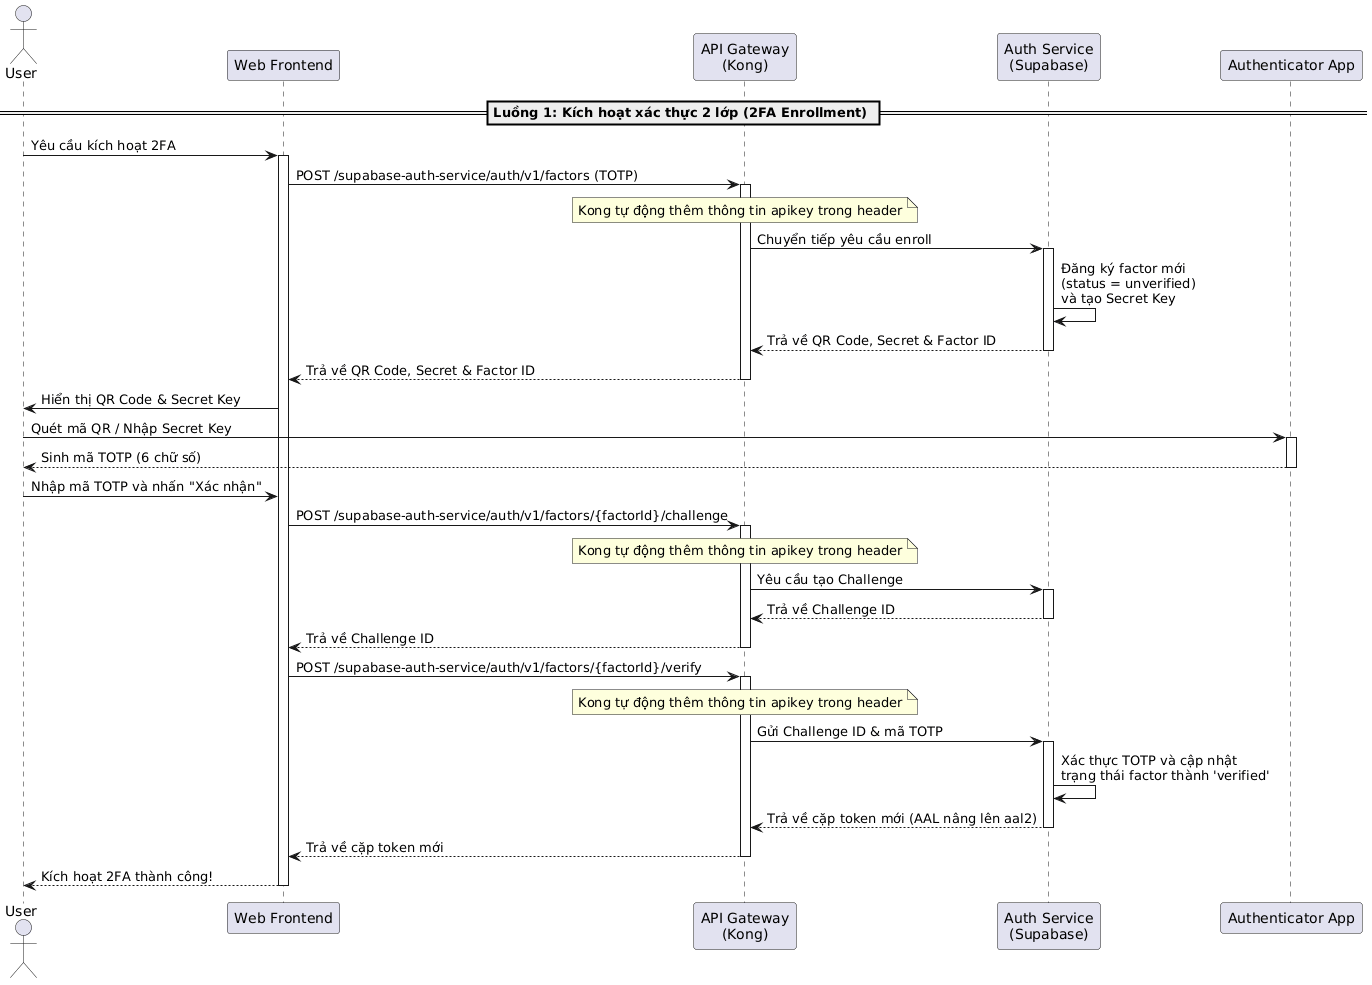
\includegraphics[scale = 0.3]{contents/Sequence/UML-Sequence-UserMfaEnrollment.png}
\caption{Sơ đồ tuần tự luồng Kích hoạt xác thực 2 lớp}
\end{figure}

\subparagraph{Các thành phần tham gia}

\begin{table}[H]
\centering
\renewcommand{\arraystretch}{1.3}

\begin{tabular}{|l|l|p{5cm}|}
\hline
\textbf{Thành phần} & \textbf{Phân loại} & \textbf{Vai trò trong hệ thống} \\ \hline
User & Actor & Người dùng thực hiện kích hoạt xác thực 2 lớp. \\ \hline
Web Frontend & Component & Giao diện web Next.js. \\ \hline
API Gateway (Kong) & Component & Cổng API chuyển tiếp các yêu cầu API. \\ \hline
Auth Service (Supabase) & Microservice & Dịch vụ xác thực sinh mã bí mật và xác minh TOTP. \\ \hline
Authenticator App & External Service & Ứng dụng di động (Google Authenticator...) quét QR sinh mã TOTP. \\ \hline
\end{tabular}
\caption{Các thành phần tham gia luồng Kích hoạt xác thực 2 lớp}
\end{table}

\subparagraph{Mô tả tổng quan}

\begin{itemize}
\item User chọn kích hoạt 2FA. Frontend gọi API \texttt{POST /factors} qua Gateway (Kong) đến Auth Service. Auth Service thực hiện đăng ký yếu tố xác thực mới ở trạng thái chưa kiểm chứng (\texttt{unverified}) và sinh thông tin khóa bí mật cùng mã QR Code để trả về.
\item User quét mã QR bằng Authenticator App để cấu hình đồng bộ. Ứng dụng này sẽ sinh mã TOTP cập nhật liên tục mỗi 30 giây.
\item User nhập TOTP thử nghiệm. Frontend gửi yêu cầu qua Gateway để tạo mã thách thức (\texttt{POST /factors/\{id\}/challenge}) và gửi mã TOTP kèm mã thách thức để xác thực kích hoạt (\texttt{POST /factors/\{id\}/verify}).
\item Nếu mã TOTP chính xác, Auth Service xác thực và kích hoạt trạng thái \texttt{verified} cho thiết bị xác thực, đồng thời cấp lại Access Token mới nâng cấp mức độ bảo mật lên \texttt{aal2}.
\end{itemize}
